\section{Modélisations des traitements}
Commentaire.  La modélisation des traitements est composée de la modélisation fonctionnelle et de la modélisation dynamiques.  TOUTES les rubriques ci-dessous doivent être complétées.  Si vous n’utilisez pas la notation UML, vous utilisez un diagramme de flux de données (DFD).

subsection{Liste des acteurs humains et non-humains}
Commentaire.  Les acteurs sont les entités externes qui sont en interactions avec l’application.  TOUS les acteurs doivent être listés ET documentés.

\subsection{Diagramme de cas d’utilisation (UML)}
Commentaire.  Indiquez tous les traitements nécessaires et suffisants pour répondre aux demandes du client ci-dessus. Le niveau de détail doit être suffisant pour que le programmeur puisse développer les composants.

Attention :  TOUS les cas d’utilisation doivent impérativement être documentés de telle manière que le programmeur dispose de toutes les informations pour développer les composants.



\begin{center}
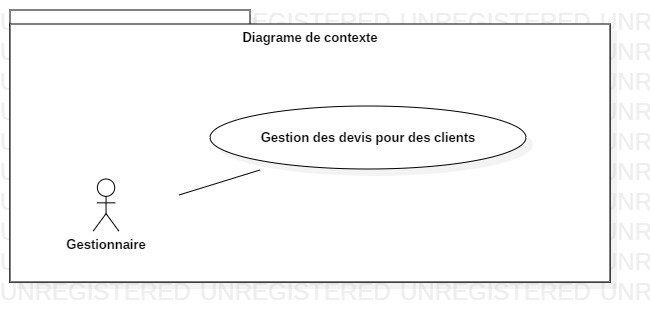
\includegraphics[scale=0.7]{use_case/contexte.jpg} 
\end{center}

\begin{center}
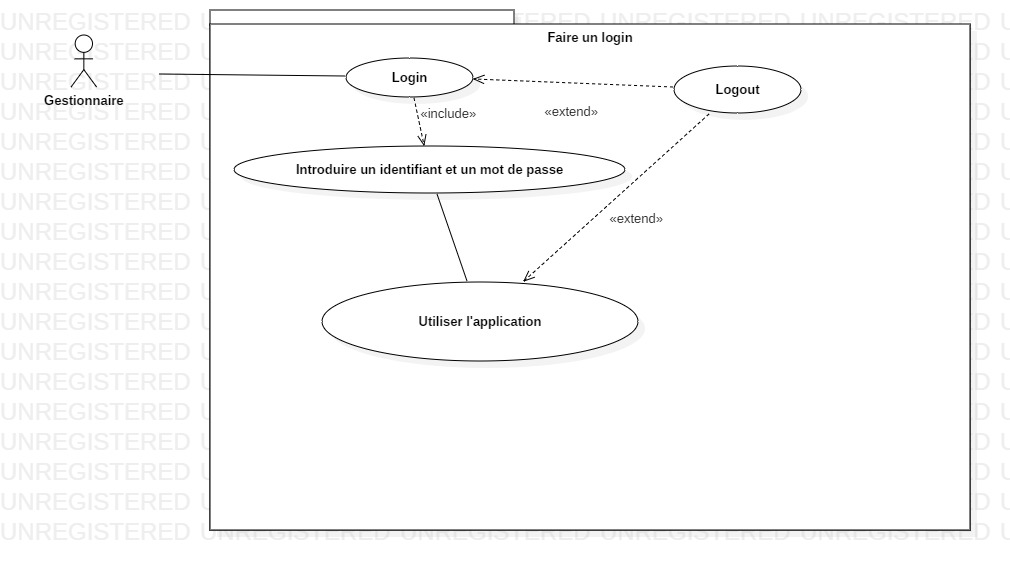
\includegraphics[scale=0.5]{use_case/login.jpg}
\end{center}

\begin{center}
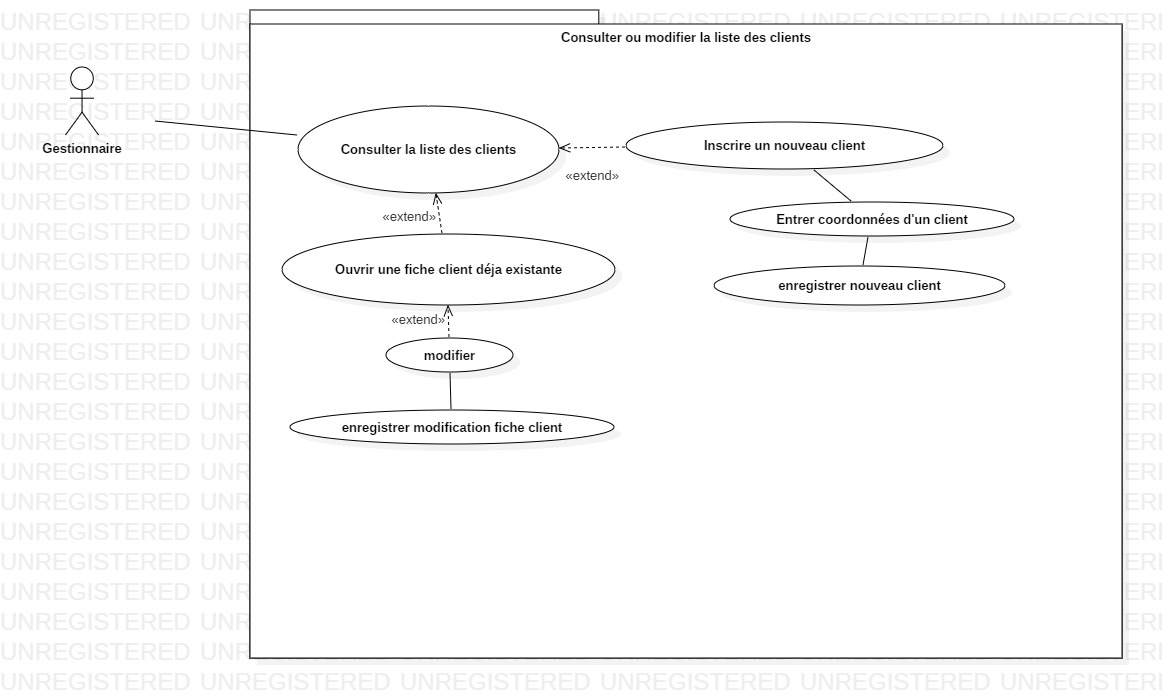
\includegraphics[scale=0.4]{use_case/consulterOuModifierListeClient.jpg} 
\end{center}

\begin{center}
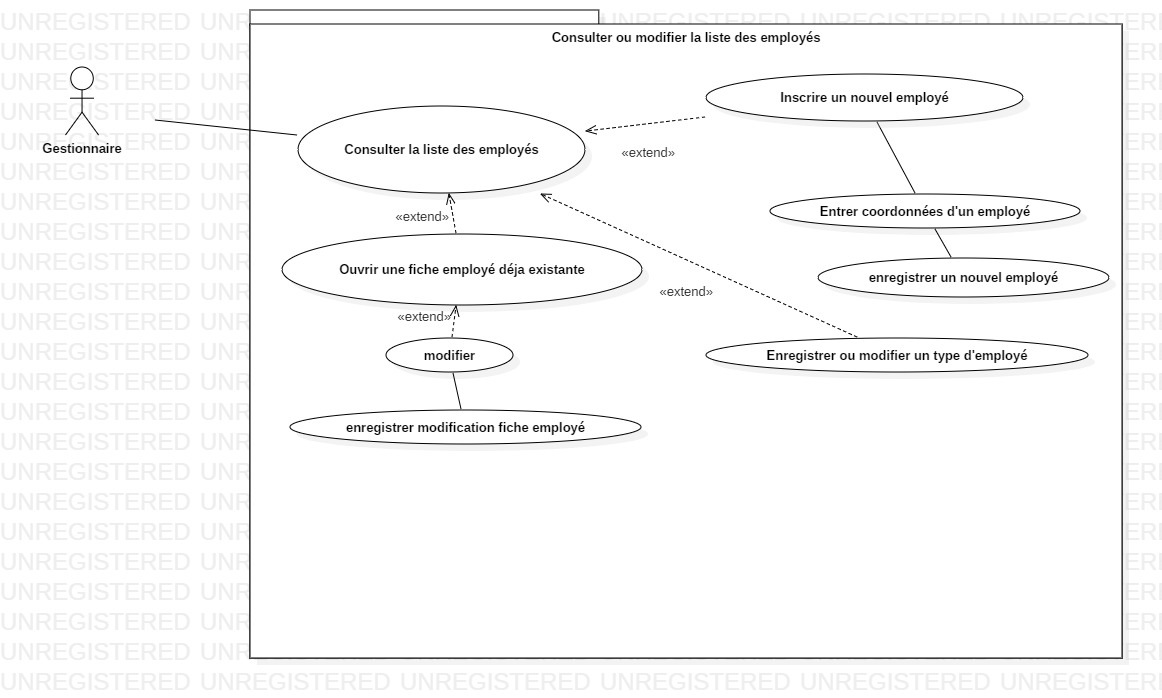
\includegraphics[scale=0.4]{use_case/consulterOuModifierListeEmploye.jpg} 
\end{center}

\begin{center}
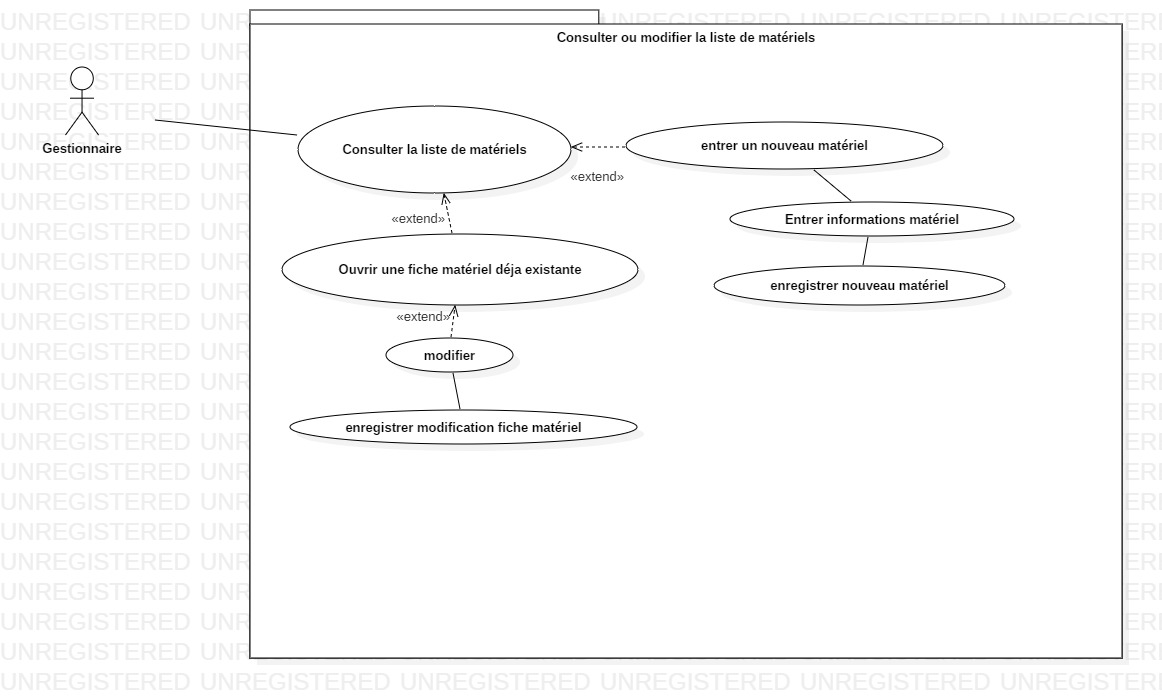
\includegraphics[scale=0.4]{use_case/consulterOuModifierListeMateriel.jpg} 
\end{center}

\begin{center}
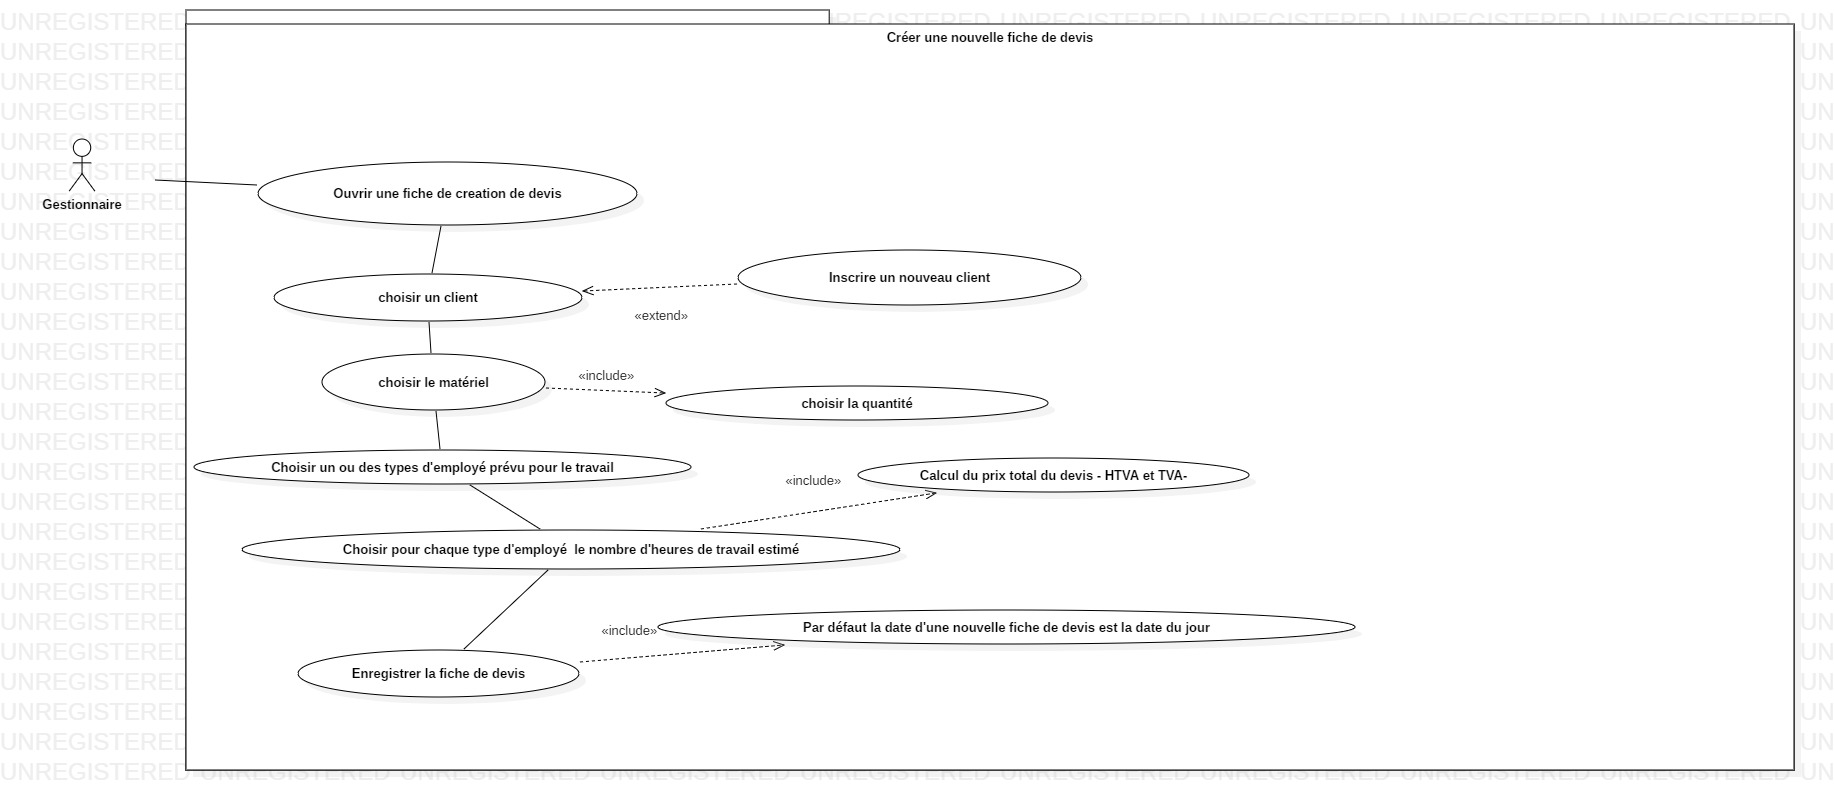
\includegraphics[scale=0.25]{use_case/ouvrirNouvelleFicheDevis.jpg} 
\end{center}

\subsection{Diagramme de séquence (UML)}
Commentaire.  Le diagramme de séquence donne la dynamique des échanges entre les acteurs, les composants du programme.

